\section{Tiến độ thực hiện giai đoạn 1 và kế hoạch giai đoạn 2}

\subsection{Tổng kết tiến độ 15 tuần của giai đoạn 1 (DACN)}
Để bảo đảm tính minh bạch và trung thực đối chiếu giữa kế hoạch đề ra ban đầu với mã nguồn thực tế tại thời điểm kết thúc Giai đoạn 1 (DACN), Bảng \ref{tab:stage1_progress} đối chiếu chi tiết từng tuần công việc theo ba trạng thái: \textbf{Hoàn thành}, \textbf{Mở rộng vượt kế hoạch} (các hướng nghiên cứu chuyên sâu đã hiện thực và kiểm chứng trong repo) và \textbf{Chuyển sang Giai đoạn 2 (DATN)} (các tính năng mang tính vận hành sản phẩm quy mô lớn).

\begin{longtable}{C{1.3cm} L{5.4cm} L{5.5cm} C{2.6cm}}
    \caption{Đối chiếu kế hoạch thực hiện 15 tuần giai đoạn 1 (DACN) với kết quả thực tế}
    \label{tab:stage1_progress} \\
    \toprule
    \textbf{Tuần} & \textbf{Kế hoạch đề ra (Giai đoạn 1)} & \textbf{Kết quả thực tế ghi nhận trong codebase} & \textbf{Trạng thái} \\
    \midrule
    \endfirsthead
    \toprule
    \textbf{Tuần} & \textbf{Kế hoạch đề ra (Giai đoạn 1)} & \textbf{Kết quả thực tế ghi nhận trong codebase} & \textbf{Trạng thái} \\
    \midrule
    \endhead
    \bottomrule
    \endfoot

    Tuần 1 & Dựng bản mẫu bàn cờ $6 \times 6$, AP, di chuyển, hợp thể, sinh vật cản ngẫu nhiên và kiểm tra nước đi. & Hoàn thiện nhân C\# thuần: \texttt{GameState}, \texttt{MoveValidator}, \texttt{PassiveFlags} (9-bit), sinh $1$--$2$ vật cản trung tuyến, Surge Phase. & Hoàn thành \\
    \midrule
    Tuần 2 & Tách cấu hình, PvP Offline, highlight/rung/zoom camera và Minimax Alpha-Beta cơ bản. & Hoàn thiện \texttt{GameConfig} ScriptableObject, \texttt{PvPOffModeBootstrapper}, \texttt{BoardRotator}, \texttt{CamShaked}/\texttt{ZoomCam}, \texttt{MinimaxSearch}. & Hoàn thành \\
    \midrule
    Tuần 3 & Squad Builder $10$ Slots, điều kiện kết thúc, mô phỏng hàng loạt tìm lỗi kẹt cờ, khảo sát Photon. & Hoàn thiện \texttt{UIPopupSquadBuilder}, \texttt{SquadValidator}, \texttt{SaveLoadManager}, tích hợp Photon Fusion 2. & Hoàn thành \\
    \midrule
    Tuần 4 & Kết nối mạng 2 máy (region, phòng, đồng bộ đội hình, timer) và bắt đầu huấn luyện ML-Agents. & Hiện thực \texttt{OnlineSessionManager}, \texttt{OnlineDataBroadcastNetwork}, \texttt{OnlineTurnTimer}, \texttt{AgentBotController} + BC/PPO. & Hoàn thành \\
    \midrule
    Tuần 5 & Thay mô hình 3D Trung cổ, dựng Scene benchmark đối kháng AI, sửa lỗi đồng bộ Ready/Tên Online. & Tích hợp 6 quân cờ 3D Medieval, hoàn thiện \texttt{BenchmarkBootstrapper} + \texttt{FileBenchmarkRecorder}, sửa đồng bộ tên/Ready. & Hoàn thành \\
    \midrule
    Tuần 6 & Thử nghiệm AI Hybrid (ML + Minimax), animation Idle/Move/Attack, dựng lại UI Main Menu/Lobby/HUD. & Hiện thực \texttt{HybridAgentBotController}, \texttt{NeuralMinimaxBotController}, FSM quân cờ và bộ giao diện UGUI qua \texttt{UIMapper}. & Hoàn thành \\
    \midrule
    Tuần 7 & Animation GetHit/Death, VFX đòn đánh, zoom camera khi ăn quân, nâng cấp bàn cờ 3D. & Hoàn thiện 5 trạng thái \texttt{PieceView}, chuẩn hóa \texttt{PieceAnimationRelay}, nâng cấp bàn cờ 3D và \texttt{PieceGhostTrail}. & Hoàn thành \\
    \midrule
    Tuần 8 & Hệ thống âm thanh SFX/BGM, cân chỉnh Skybox/ánh sáng và khởi động nghiên cứu SC (Nam/Nữ). & Hiện thực \texttt{AudioManager}, Skybox/lighting URP, chuẩn bị base mesh Nam/Nữ trên MPFB v2 (Blender 4.2). & Hoàn thành \\
    \midrule
    Tuần 9 & Thử nghiệm nắn hình học 3D từ ảnh 2D, xử lý màu da/UV và xem trước trong Unity. & Xây dựng pipeline Python FastAPI + \texttt{SCCharacterCreator}, kiểm chứng loại bỏ hướng Z-MediaPipe và \texttt{sc\_texnet}. & Hoàn thành \\
    \midrule
    Tuần 10 & Đưa giao diện SC vào game kèm thanh trượt thủ công và nghiên cứu khử bóng Texture (delighting). & Hiện thực \texttt{SCCanvasUI}, \texttt{SCBlendShapeRow}, tích hợp IC-Light FP16 ($\sim 1.8$s) và Method B1 v2 ($25$ kênh trực giao). & Hoàn thành \\
    \midrule
    Tuần 11 & Làm mượt biên cổ (seam blending), hạn chế méo UV và kiểm tra chuyển đổi Nam -- Nữ. & Hoàn thiện chiếu Barycentric PyTorch3D, Hermite $64$px, HRN Normal Map, mắt PBR Catchlight và \textbf{bổ sung 6 kiểu tóc 3D MPFB v2}. & Mở rộng vượt kế hoạch \\
    \midrule
    Tuần 12 & Mở rộng tự đấu AI, kiểm tra ổn định mạng (desync/lag); \textit{thêm tìm trận tự động, đấu hạng, Elo}. & Hoàn thiện \textbf{NNUE, Residual NNUE ($51\%$ thắng D4), ObservationEncoderV2 ($654$f) và LLM Evolved Module Bank}; chạy benchmark $10$ probes mạng. Hạng mục Matchmaking/Elo dời sang DATN. & Mở rộng AI; dời Elo sang DATN \\
    \midrule
    Tuần 13 & Mô phỏng cân bằng đi trước/đi sau, rà soát tình huống biên AP/Hợp thể, VFX; \textit{bảng xếp hạng, bạn bè}. & Xử lý race condition Attack/Move, kiểm thử hàng trăm ván tự đấu AI; hoàn thiện bộ VFX sấm sét/va chạm. Hạng mục Bảng xếp hạng và Bạn bè dời sang DATN. & Hoàn thành Core/AI; dời Social sang DATN \\
    \midrule
    Tuần 14 & Ghép luồng cài đặt, thử nghiệm lưu dữ liệu, đo hiệu năng khung hình và bộ nhớ. & Hoàn thiện \texttt{UIPopupSettings}, \texttt{SaveLoadManager} (\texttt{SquadSLO}, \texttt{GeneralSettingsSLO}), kiểm tra tốc độ suy nghĩ AI ($<70$ ms). & Hoàn thành cơ bản \\
    \midrule
    Tuần 15 & Chơi thử tìm lỗi góc chết, tổng hợp danh sách lỗi và dựng bản cài đặt mẫu PC. & Tổng hợp danh sách lỗi/hạn chế cho Giai đoạn 2, hoàn thiện tài liệu kiến trúc và báo cáo tổng kết Giai đoạn 1 (DACN). & Hoàn thành \\
\end{longtable}

\subsection{Tổng kết đóng góp của từng thành viên trong giai đoạn 1}
Bảng \ref{tab:member_contrib} ghi nhận đóng góp thực tế của hai thành viên căn cứ theo lịch sử commit Git (tổng cộng hơn $260$ commit tính đến tháng 11/2026).

\begin{table}[H]
    \centering
    \caption{Bảng tổng kết phân công và đóng góp của thành viên trong giai đoạn 1 (DACN)}
    \label{tab:member_contrib}
    \begin{tabularx}{\textwidth}{L{3.2cm} Y C{2.2cm}}
        \toprule
        \textbf{Thành viên} & \textbf{Các hạng mục kỹ thuật chủ trì và hoàn thành} & \textbf{Tỷ trọng} \\
        \midrule
        Thành viên 1 (Chủ trì Core, AI và SC) & Kiến trúc Hexagonal và \texttt{ArenaServiceLocator}; toàn bộ Core Domain (\texttt{GameState}, \texttt{MoveValidator}, \texttt{MatchManager}, \texttt{PassiveFlags}); toàn bộ hệ sinh thái AI (Minimax/PVS/Zobrist, BC/DAgger, PPO Self-Play, \texttt{ObservationEncoderV2}, NNUE/Residual NNUE, Hybrid Bot, LLM FunSearch); toàn bộ pipeline Smart Customization (Method B1 v2, IC-Light, PyTorch3D, HRN, 3D Hair, PBR Eyes); \texttt{PieceAnimationRelay} và hệ thống Benchmark tự động. & 50\% \\
        \midrule
        Thành viên 2 -- Đăng (Chủ trì Multiplayer và View Layer) & Khảo sát và triển khai Multiplayer trên Photon Fusion (\texttt{OnlineSessionManager}, \texttt{OnlineDataBroadcastNetwork}, 9 \texttt{BroadcastDataHandler}, \texttt{NetworkController}, \texttt{OnlineLocalMoveSender}, \texttt{OnlineTurnTimer}, đo benchmark NetworkObject vs Reliable Data); PvP Offline (\texttt{BoardRotator}); tầng View (\texttt{BoardView}, \texttt{TileView}, \texttt{PieceView} 3D, \texttt{VisualQueueManager}); toàn bộ hệ thống UI (\texttt{UIManager}, \texttt{UIMapper}, \texttt{UIPopupSquadBuilder}, \texttt{UIPopupLobby}, \texttt{UIInGameHUD}); tích hợp VFX/SFX và Skybox. & 50\% \\
        \bottomrule
    \end{tabularx}
\end{table}

\subsection{Đánh giá chung và các hạn chế còn tồn tại}
Kết thúc Giai đoạn 1 (DACN), nhóm đã chứng minh trọn vẹn tính khả thi kỹ thuật của cả bốn mảng phức tạp nhất: lõi cờ chiến thuật $6 \times 6$ tách rời hoàn toàn khỏi Unity, AI lai \texttt{Residual NNUE} vượt trội Heuristic Depth 4 ở thời gian phản hồi $66$ ms, giao thức mạng nhị phân 4-byte trên Photon Fusion tiết kiệm $78.1\%$ băng thông và pipeline tạo khuôn mặt/tóc 3D từ ảnh chân dung chạy thực tế trên GPU tầm trung.

Tuy nhiên, do phạm vi DACN tập trung vào khảo sát, kiến trúc và nguyên mẫu, sản phẩm hiện vẫn còn năm hạn chế chính cần giải quyết triệt để ở Giai đoạn 2:
\begin{enumerate}
    \item \textbf{Chưa hoàn thiện xử lý sự cố mạng và tài khoản người chơi:} Hệ thống Multiplayer hiện chưa có cơ chế tự động kết nối lại (Reconnect) sau khi đứt mạng giữa trận, chưa xử lý triệt để mọi tình huống hết giờ/rời phòng đột ngột và chưa tích hợp xác thực tài khoản (Google/Facebook) hay cơ sở dữ liệu đám mây.
    \item \textbf{Chưa có hệ thống cạnh tranh xã hội:} Các tính năng ghép trận tự động (Matchmaking), tính điểm xếp hạng Elo, bảng xếp hạng toàn cục (Leaderboard) và danh sách bạn bè mới dừng ở mức thiết kế kế hoạch.
    \item \textbf{Triển khai Smart Customization còn phụ thuộc môi trường Python cục bộ:} Backend FastAPI hiện chạy trên máy trạm phát triển có GPU RTX 4050; cần phương án đóng gói dịch vụ hoặc triển khai máy chủ suy luận (hoặc rút gọn ONNX chạy trực tiếp trên thiết bị) khi phát hành cho người dùng cuối.
    \item \textbf{Chưa cài đặt quy tắc hòa lặp thế cờ 3 lần (Threefold Repetition):} Hiện chỉ mới giới hạn hòa theo \texttt{MaxTurns = 60} và giới hạn lượt Pass.
    \item \textbf{Chưa tiến hành tối ưu hiệu năng sâu và kiểm thử người dùng quy mô lớn:} Chưa tối ưu Draw Calls/GPU Instancing, chưa có hướng dẫn tân thủ tương tác (Interactive Tutorial) cho luật hợp thể + Surge và chưa thu thập dữ liệu khảo sát trải nghiệm từ người chơi thực tế.
\end{enumerate}

\subsection{Kế hoạch triển khai giai đoạn 2 -- Đồ án tốt nghiệp (DATN)}
Nếu Giai đoạn 1 (DACN) là chặng \textit{nghiên cứu, đánh giá và chứng minh nguyên mẫu}, thì \textbf{Giai đoạn 2 (DATN -- dự kiến 16 tuần, từ Tuần 16 đến Tuần 31)} hướng thẳng tới mục tiêu \textbf{hoàn thiện sản phẩm đạt chất lượng phát hành công khai (Production-ready Release)} trên nền tảng PC (itch.io / Steam Demo). Hình \ref{fig:roadmap_gantt} và Bảng \ref{tab:stage2_plan} mô tả lộ trình chuyển tiếp liền mạch giữa hai giai đoạn.

\begin{figure}[H]
    \centering
    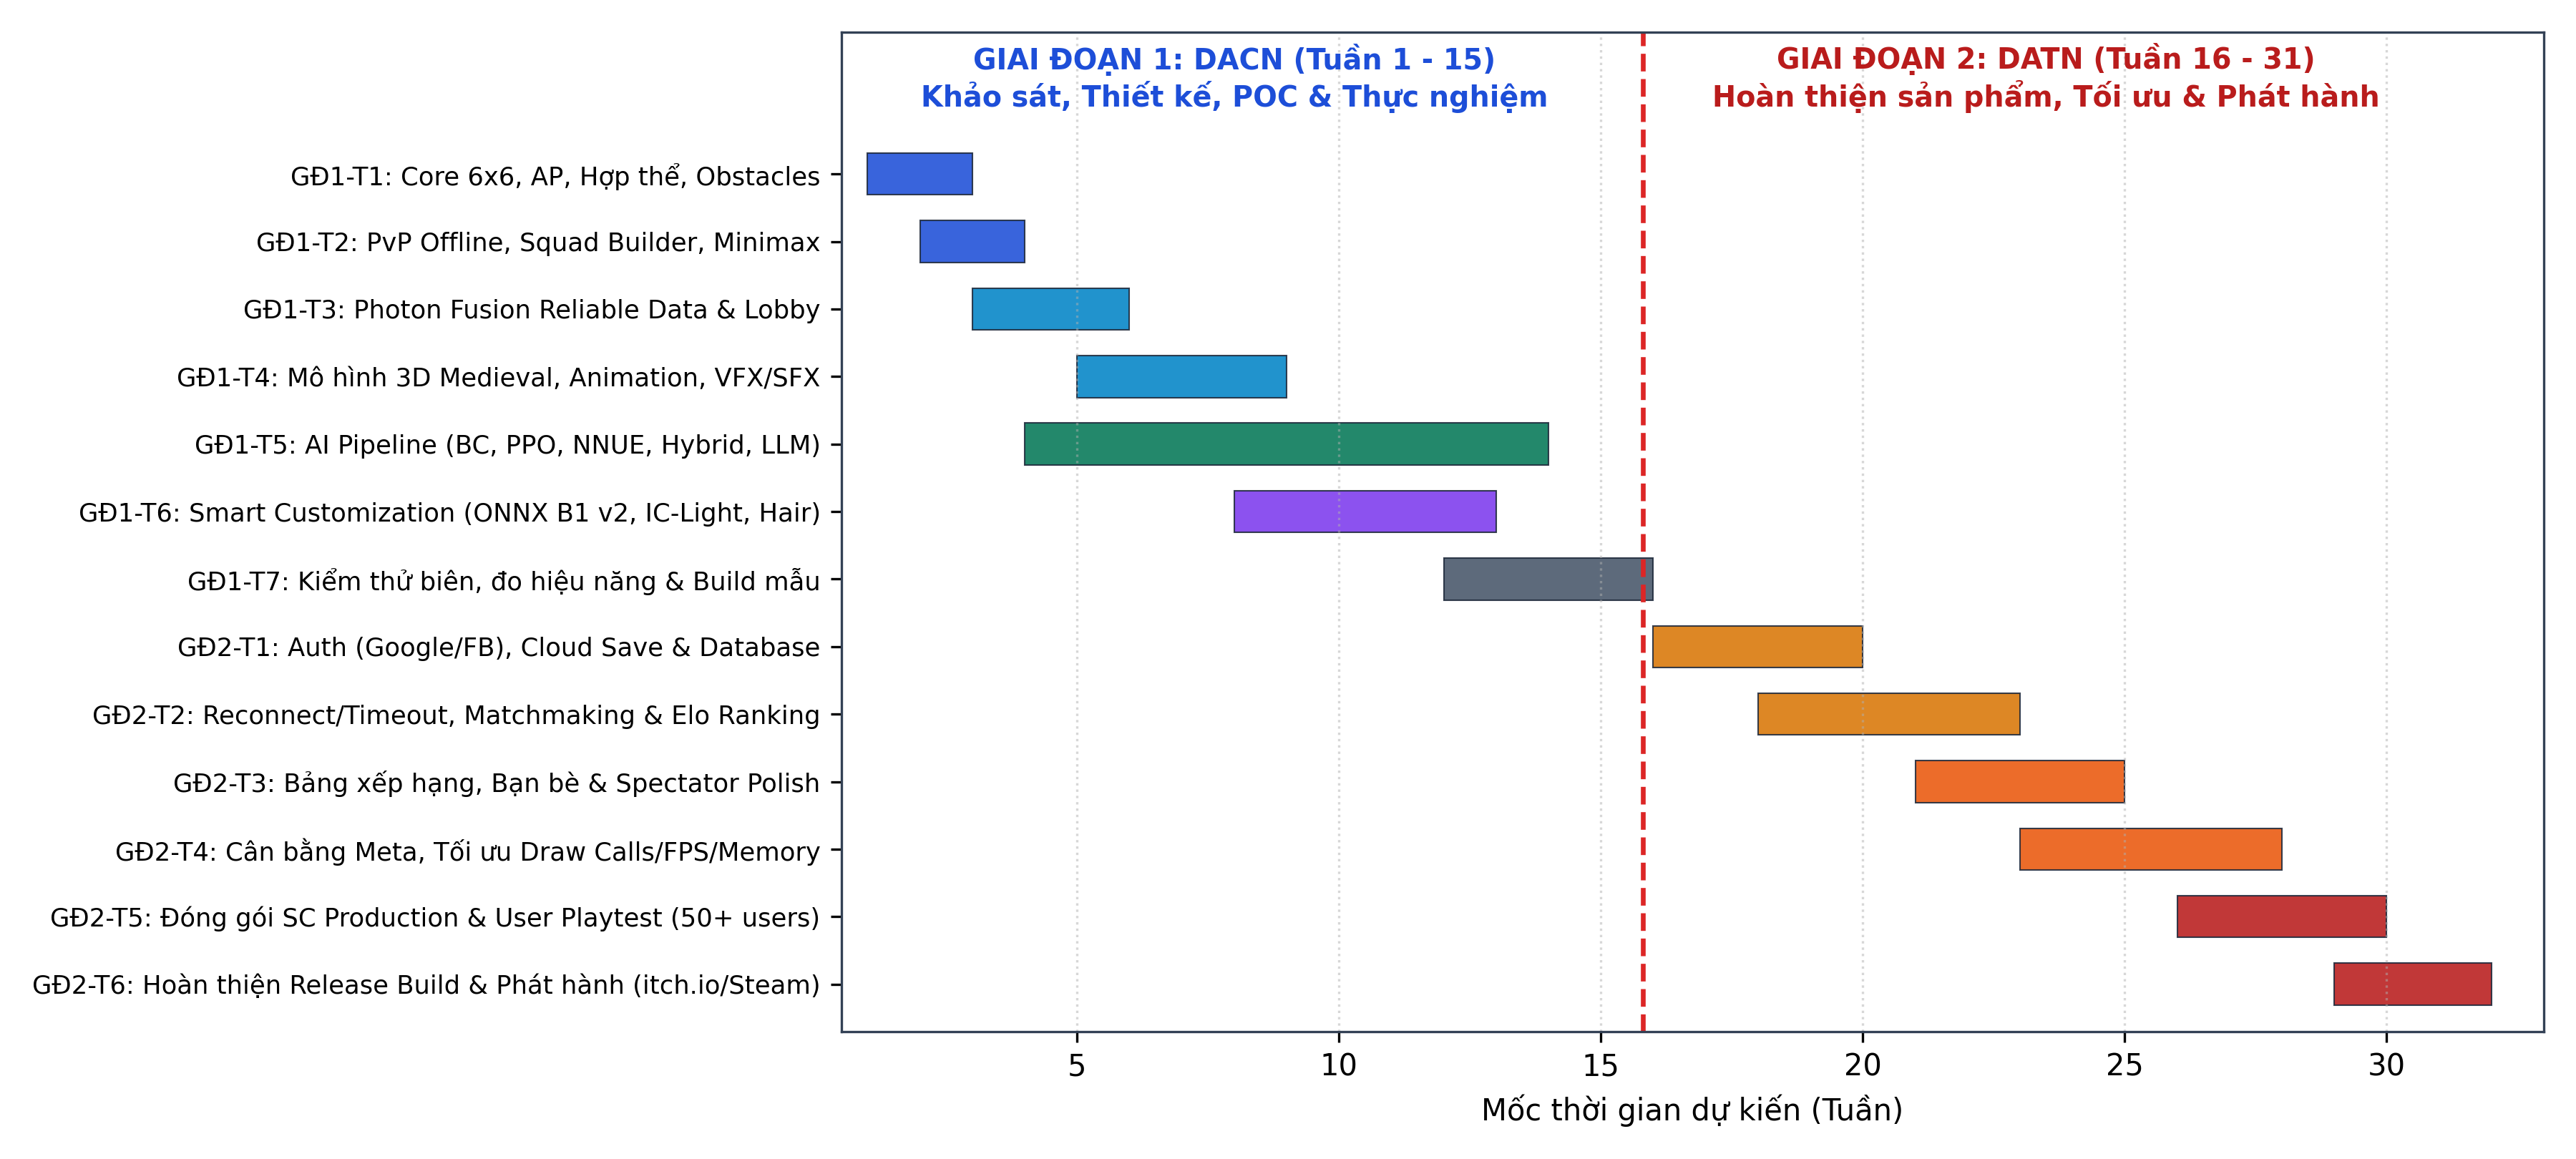
\includegraphics[width=\textwidth]{Diagrams/images/chart_roadmap_gantt.png}
    \caption{Lộ trình tổng thể hai giai đoạn từ Đồ án chuyên ngành (Tuần 1--15) sang Đồ án tốt nghiệp (Tuần 16--31)}
    \label{fig:roadmap_gantt}
\end{figure}

{\small
\begin{longtable}{L{2.5cm} L{2.0cm} L{5.7cm} L{4.7cm}}
    \caption{Kế hoạch chi tiết triển khai giai đoạn 2 (Đồ án tốt nghiệp -- DATN) hướng tới hoàn thiện và phát hành}
    \label{tab:stage2_plan} \\
    \toprule
    \textbf{Giai đoạn con} & \textbf{Mốc thời gian} & \textbf{Hạng mục công việc trọng tâm} & \textbf{Sản phẩm đầu ra (Deliverables)} \\
    \midrule
    \endfirsthead
    \toprule
    \textbf{Giai đoạn con} & \textbf{Mốc thời gian} & \textbf{Hạng mục công việc trọng tâm} & \textbf{Sản phẩm đầu ra (Deliverables)} \\
    \midrule
    \endhead
    \bottomrule
    \endfoot
        Pha 2.1: Hạ tầng tài khoản và dữ liệu đám mây & Tuần 16 -- 19 & Tích hợp đăng nhập Firebase Auth / Google / Facebook; thiết kế CSDL đám mây (Firestore / PlayFab) lưu hồ sơ người chơi, đội hình, lịch sử đấu và tham số avatar SC. & Hệ thống tài khoản đa thiết bị, Cloud Save thay thế lưu cục bộ đơn lẻ, lược đồ ERD hoàn chỉnh. \\
        \midrule
        Pha 2.2: Ổn định mạng, Matchmaking và Elo & Tuần 18 -- 22 & Hoàn thiện xử lý timeout, grace period và cơ chế Reconnect đồng bộ lại toàn bộ \texttt{GameState}; xây dựng hàng đợi ghép trận tự động (Matchmaking) và thuật toán tính điểm Elo; cân nhắc nâng cấp kiến trúc kiểm soát chống gian lận phía server (Authoritative Validation). & Chế độ Đấu hạng (Ranked PvP Online) ổn định trước sự cố ngắt mạng; vượt qua kiểm thử mô phỏng rớt gói $5\%$--$10\%$. \\
        \midrule
        Pha 2.3: Hệ thống xã hội và hoàn thiện luật chơi & Tuần 21 -- 24 & Xây dựng Bảng xếp hạng (Leaderboard), Danh sách bạn bè (mời đấu trực tiếp), xem lại đội hình người chơi; hoàn thiện luật hòa lặp thế cờ 3 lần (Zobrist History) và chế độ Khán giả nâng cao (Replay/Spectator HUD). & Màn hình Leaderboard, Friends System, Match History và bộ luật chuẩn giải đấu không còn tình huống biên mở. \\
        \midrule
        Pha 2.4: Cân bằng Meta AI, tối ưu hóa và hướng dẫn & Tuần 23 -- 27 & Phân tầng độ khó Bot PvE (Dễ: Heuristic D1/D2; Trung bình: PPO/NeuralMinimax; Khó: Residual NNUE / Hybrid / LLM); chạy mô phỏng $10{,}000+$ ván cân bằng tỷ lệ thắng đi trước/đi sau và chi phí AP/Slot; tối ưu Draw Calls (Static/GPU Batching, LOD, Object Pooling VFX), kiểm soát Memory/GC; xây dựng Interactive Tutorial. & Báo cáo profiling trước/sau tối ưu ($\ge 60$ FPS ổn định trên máy cấu hình thấp); bộ 4 cấp độ AI phục vụ người chơi; màn hướng dẫn tân thủ. \\
        \midrule
        Pha 2.5: Đóng gói SC, Playtest và phát hành & Tuần 26 -- 31 & Đóng gói dịch vụ Smart Customization (Docker GPU Cloud API hoặc chế độ Fallback nhẹ khi ngoại tuyến); tổ chức kiểm thử người dùng (Closed/Open Beta với $\ge 50$ người chơi) thu thập telemetry và bảng hỏi UX (SUS/GEQ); sửa lỗi cuối cùng và phát hành bản cài đặt Windows hoàn chỉnh. & Bản phát hành công khai trên itch.io / Steam Demo; tập dữ liệu khảo sát người dùng và báo cáo khóa luận tốt nghiệp hoàn chỉnh. \\
\end{longtable}
}
